%package list
\documentclass{article}
\usepackage[top=3cm, bottom=3cm, outer=3cm, inner=3cm]{geometry}
\usepackage{multicol}
\usepackage{graphicx}
\usepackage{url}
%\usepackage{cite}
\usepackage{hyperref}
\usepackage{array}
%\usepackage{multicol}
\newcolumntype{x}[1]{>{\centering\arraybackslash\hspace{0pt}}p{#1}}
\usepackage{natbib}
\usepackage{pdfpages}
\usepackage{multirow}
\usepackage[normalem]{ulem}
\useunder{\uline}{\ul}{}
\usepackage{svg}
\usepackage{xcolor}
\usepackage{listings}
\usepackage{enumitem}
\usepackage{amsmath}
\lstdefinestyle{ascii-tree}{
    literate={├}{|}1 {─}{--}1 {└}{+}1 
  }
\lstset{basicstyle=\ttfamily,
  showstringspaces=false,
  commentstyle=\color{red},
  keywordstyle=\color{blue}
}
%\usepackage{booktabs}
\usepackage{caption}
\usepackage{subcaption}
\usepackage{float}
\usepackage{array}

\newcolumntype{M}[1]{>{\centering\arraybackslash}m{#1}}
\newcolumntype{N}{@{}m{0pt}@{}}


%%%%%%%%%%%%%%%%%%%%%%%%%%%%%%%%%%%%%%%%%%%%%%%%%%%%%%%%%%%%%%%%%%%%%%%%%%%%
%%%%%%%%%%%%%%%%%%%%%%%%%%%%%%%%%%%%%%%%%%%%%%%%%%%%%%%%%%%%%%%%%%%%%%%%%%%%
\newcommand{\itemStudent}{%
    \begin{minipage}[t]{0.9\linewidth}
        - David Alfredo Huamani Ollachica \\
        - Marco Antonio Suarez Huamaní \\
        - Rafael Diego Nina Calizaya \\
        - Angel Paul Apaza Nazareth
    \end{minipage}%
}

\newcommand{\itemCourse}{Programación Web 2}
\newcommand{\itemCourseCode}{1702122}
\newcommand{\itemSemester}{III}
\newcommand{\itemUniversity}{Universidad Nacional de San Agustín de Arequipa}
\newcommand{\itemFaculty}{Facultad de Ingeniería de Producción y Servicios}
\newcommand{\itemDepartment}{Departamento Académico de Ingeniería de Sistemas e Informática}
\newcommand{\itemSchool}{Escuela Profesional de Ingeniería de Sistemas }
\newcommand{\itemAcademic}{2024 - A}
\newcommand{\itemInput}{Del 7 Junio 2024}
\newcommand{\itemOutput}{Al 14 Junio 2024}
\newcommand{\itemPracticeNumber}{07}
\newcommand{\itemTheme}{Django (Modelos, Vistas y Templates)}
%%%%%%%%%%%%%%%%%%%%%%%%%%%%%%%%%%%%%%%%%%%%%%%%%%%%%%%%%%%%%%%%%%%%%%%%%%%%
%%%%%%%%%%%%%%%%%%%%%%%%%%%%%%%%%%%%%%%%%%%%%%%%%%%%%%%%%%%%%%%%%%%%%%%%%%%%

\usepackage[english,spanish]{babel}
\usepackage[utf8]{inputenc}
\AtBeginDocument{\selectlanguage{spanish}}
\renewcommand{\figurename}{Figura}
\renewcommand{\refname}{Referencias}
\renewcommand{\tablename}{Tabla} %esto no funciona cuando se usa babel
\AtBeginDocument{%
	\renewcommand\tablename{Tabla}
}

\usepackage{fancyhdr}
\pagestyle{fancy}
\fancyhf{}
\setlength{\headheight}{30pt}
\renewcommand{\headrulewidth}{1pt}
\renewcommand{\footrulewidth}{1pt}
\fancyhead[L]{\raisebox{-0.2\height}{
\includegraphics[width=3cm]{img/logo_episunsa.png}}}
\fancyhead[C]{\fontsize{7}{7}\selectfont	\itemUniversity \\ \itemFaculty \\ \itemDepartment \\ \itemSchool \\ \textbf{\itemCourse}}
\fancyhead[R]{\raisebox{-0.2\height}{
\includegraphics[width=1.2cm]{img/logo_abet}}}
\fancyfoot[L]{Grupo 3 - PW2}
\fancyfoot[C]{\itemCourse}
\fancyfoot[R]{Página \thepage}

% para el codigo fuente
\usepackage{listings}
\usepackage{color, colortbl}
\definecolor{dkgreen}{rgb}{0,0.6,0}
\definecolor{gray}{rgb}{0.5,0.5,0.5}
\definecolor{mauve}{rgb}{0.58,0,0.82}
\definecolor{codebackground}{rgb}{0.95, 0.95, 0.92}
\definecolor{tablebackground}{rgb}{0.8, 0, 0}

\lstset{frame=tb,
	language=Python,
	aboveskip=3mm,
	belowskip=3mm,
	showstringspaces=false,
	columns=flexible,
	basicstyle={\small\ttfamily},
	numbers=none,
	numberstyle=\tiny\color{gray},
	keywordstyle=\color{blue},
	commentstyle=\color{dkgreen},
	stringstyle=\color{mauve},
	breaklines=true,
	breakatwhitespace=true,
	tabsize=4,
	backgroundcolor= \color{codebackground},
}

\begin{document}
	
	\vspace*{10px}
	
	\begin{center}	
		\fontsize{17}{17} \textbf{ Informe de Laboratorio \itemPracticeNumber}
	\end{center}
	\centerline{\textbf{\Large Tema: \itemTheme}}
	%\vspace*{0.5cm}	

	\begin{flushright}
		\begin{tabular}{|M{2.5cm}|N|}
			\hline 
			\rowcolor{tablebackground}
			\color{white} \textbf{Nota}  \\
			\hline 
			     \\[30pt]
			\hline 			
		\end{tabular}
	\end{flushright}	

	\begin{table}[H]
		\begin{tabular}{|x{4.7cm}|x{4.8cm}|x{4.8cm}|}
			\hline 
			\rowcolor{tablebackground}
			\color{white} \textbf{Estudiante} & \color{white}\textbf{Escuela}  & \color{white}\textbf{Asignatura}   \\
			\hline 
			{\itemStudent } & \itemSchool & {\itemCourse \par Semestre: \itemSemester \par Código: \itemCourseCode}     \\ 
			\hline 			
		\end{tabular}
	\end{table}		
	
	\begin{table}[H]
		\begin{tabular}{|x{4.7cm}|x{4.8cm}|x{4.8cm}|}
			\hline 
			\rowcolor{tablebackground}
			\color{white}\textbf{Laboratorio} & \color{white}\textbf{Tema}  & \color{white}\textbf{Duración}   \\
			\hline 
			\itemPracticeNumber & \itemTheme & 04 horas   \\
			\hline 
		\end{tabular}
	\end{table}
	
	\begin{table}[H]
		\begin{tabular}{|x{4.7cm}|x{4.8cm}|x{4.8cm}|}
			\hline 
			\rowcolor{tablebackground}
			\color{white}\textbf{Semestre académico} & \color{white}\textbf{Fecha de inicio}  & \color{white}\textbf{Fecha de entrega}   \\
			\hline 
			\itemAcademic & \itemInput &  \itemOutput  \\
			\hline 
		\end{tabular}
	\end{table}
	
	\section{Tarea}
	
\begin{itemize}
    \item URL GitHub del Projecto Django \url{https://github.com/Suarezsh/Lab7}   
    \item Se usa solo una aplicacion en todo el proyecto, esta aplicacion se llama sistemaAcademico
                \begin{figure}[h]
                \centering
                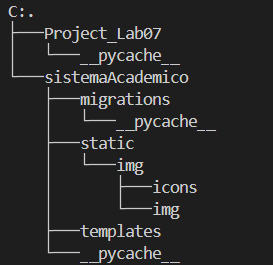
\includegraphics[width=0.3\textwidth]{img/tree.png}
                \caption{Arbol de carpetas y archivos del proyecto}
                \label{fig:modelo_bd}
            \end{figure}
            
\end{itemize}


	\section{Modelos}
	
	\subsection{Diagrama E - R de los modelos usados para la practica}
                \begin{figure}[h]
                \centering
                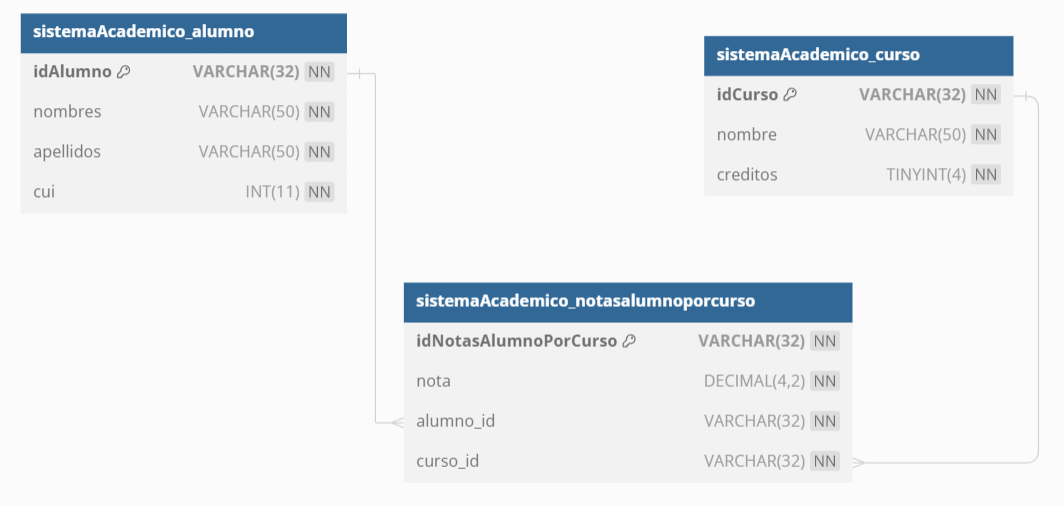
\includegraphics[width=0.9\textwidth]{img/models.png}
                \caption{Diagrama de la base de datos}
                \label{fig:modelo_bd}
            \end{figure}

  
\subsection{Modelos en código Python}
\begin{itemize}
    \item El código define tres modelos en Django para gestionar información de alumnos, cursos y las notas de los alumnos en dichos cursos. A continuación, se describen brevemente los modelos:
\end{itemize}

\begin{itemize}
    \item \textbf{Modelo Alumno}:
    \begin{itemize}
        \item \texttt{idAlumno}: Un identificador único del alumno (campo clave primaria).
        \item \texttt{nombres}: El nombre del alumno.
        \item \texttt{apellidos}: El apellido del alumno.
        \item \texttt{cui}: Un campo entero para un identificador adicional del alumno (presumiblemente un número de identificación único).
    \end{itemize}

    \item \textbf{Modelo Curso}:
    \begin{itemize}
        \item \texttt{idCurso}: Un identificador único del curso (campo clave primaria).
        \item \texttt{nombre}: El nombre del curso.
        \item \texttt{creditos}: Un campo entero que representa los créditos del curso.
    \end{itemize}

    \item \textbf{Modelo NotasAlumnoPorCurso}:
    \begin{itemize}
        \item \texttt{idNotasAlumnoPorCurso}: Un identificador único para las notas (campo clave primaria).
        \item \texttt{nota}: Un campo decimal que representa la nota obtenida por el alumno en el curso.
        \item \texttt{alumno}: Una clave foránea que referencia al modelo \texttt{Alumno}.
        \item \texttt{curso}: Una clave foránea que referencia al modelo \texttt{Curso}.
    \end{itemize}
\end{itemize}

Cada modelo también tiene un método que devuelve una representación en cadena de texto del objeto.

    \begin{lstlisting}[language=Python,caption={models.py}][H]
from django.db import models
from django.utils.translation import gettext_lazy as _
class Alumno(models.Model):
    idAlumno = models.CharField(max_length=32, primary_key=True)
    nombres = models.CharField(max_length=100)
    apellidos = models.CharField(max_length=100)
    cui = models.IntegerField()
    def __str__(self):
        return f"{self.nombres} {self.apellidos}"
class Curso(models.Model):
    idCurso = models.CharField(max_length=32, primary_key=True)
    nombre = models.CharField(max_length=100)
    creditos = models.IntegerField()
    def __str__(self):
        return self.nombre
class NotasAlumnoPorCurso(models.Model):
    idNotasAlumnoPorCurso = models.CharField(max_length=32, primary_key=True)
    nota = models.DecimalField(max_digits=5, decimal_places=2)
    alumno = models.ForeignKey(Alumno, on_delete=models.CASCADE)
    curso = models.ForeignKey(Curso, on_delete=models.CASCADE)
    def __str__(self):
        return f"Notas de {self.alumno.nombres} en {self.curso.nombre}"

    \end{lstlisting}

            
    \section {Vistas}

\subsection{Descripcion de las vistas}
El código define varias vistas en Django para gestionar información de alumnos, cursos y las notas de los alumnos en dichos cursos. A continuación, se describen brevemente las vistas:

\begin{itemize}
    \item \texttt{index(request)}:
    \begin{itemize}
        \item Obtiene todos los objetos del modelo \texttt{Alumno}.
        \item Renderiza la plantilla \texttt{index.html} con la lista de alumnos.
    \end{itemize}

    \item \texttt{cursos(request)}:
    \begin{itemize}
        \item Obtiene todos los objetos del modelo \texttt{Curso}.
        \item Renderiza la plantilla \texttt{cursos.html} con la lista de cursos.
    \end{itemize}

    \item \texttt{notas(request)}:
    \begin{itemize}
        \item Obtiene todos los objetos del modelo \texttt{NotasAlumnoPorCurso}, seleccionando también los datos relacionados de \texttt{Alumno} y \texttt{Curso}.
        \item Obtiene todos los objetos del modelo \texttt{Alumno} y \texttt{Curso}.
        \item Renderiza la plantilla \texttt{notas.html} con la lista de notas, alumnos y cursos.
    \end{itemize}

    \item \texttt{agregar\_alumno(request)}:
    \begin{itemize}
        \item Si la solicitud es de tipo POST, procesa el formulario \texttt{AlumnoForm}.
        \item Si el formulario es válido, guarda el nuevo alumno y retorna una respuesta JSON con estado \texttt{success}.
        \item Si el formulario no es válido, retorna una respuesta JSON con estado \texttt{error} y los errores del formulario.
        \item Si la solicitud no es de tipo POST, retorna una respuesta JSON con estado \texttt{error}.
    \end{itemize}

    \item \texttt{eliminar\_alumno(request, idAlumno)}:
    \begin{itemize}
        \item Obtiene el objeto \texttt{Alumno} correspondiente al \texttt{idAlumno} proporcionado.
        \item Si la solicitud es de tipo POST, elimina el alumno y retorna una respuesta JSON con estado \texttt{success}.
        \item Si la solicitud no es de tipo POST, retorna una respuesta JSON con estado \texttt{error}.
    \end{itemize}

    \item \texttt{agregar\_curso(request)}:
    \begin{itemize}
        \item Si la solicitud es de tipo POST, procesa el formulario \texttt{CursoForm}.
        \item Si el formulario es válido, guarda el nuevo curso y retorna una respuesta JSON con estado \texttt{success}.
        \item Si el formulario no es válido, retorna una respuesta JSON con estado \texttt{error} y los errores del formulario.
        \item Si la solicitud no es de tipo POST, retorna una respuesta JSON con estado \texttt{error}.
    \end{itemize}

    \item \texttt{eliminar\_curso(request, idCurso)}:
    \begin{itemize}
        \item Obtiene el objeto \texttt{Curso} correspondiente al \texttt{idCurso} proporcionado.
        \item Si la solicitud es de tipo POST, elimina el curso y retorna una respuesta JSON con estado \texttt{success}.
        \item Si la solicitud no es de tipo POST, retorna una respuesta JSON con estado \texttt{error}.
    \end{itemize}

    \item \texttt{agregar\_nota(request)}:
    \begin{itemize}
        \item Si la solicitud es de tipo POST, procesa el formulario \texttt{NotasAlumnoPorCursoForm}.
        \item Si el formulario es válido, guarda la nueva nota y retorna una respuesta JSON con estado \texttt{success}.
        \item Si el formulario no es válido, retorna una respuesta JSON con estado \texttt{error} y los errores del formulario.
        \item Si la solicitud no es de tipo POST, retorna una respuesta JSON con estado \texttt{error}.
    \end{itemize}

    \item \texttt{eliminar\_nota(request, idNotasAlumnoPorCurso)}:
    \begin{itemize}
        \item Obtiene el objeto \texttt{NotasAlumnoPorCurso} correspondiente al \texttt{idNotasAlumnoPorCurso} proporcionado.
        \item Si la solicitud es de tipo POST, elimina la nota y retorna una respuesta JSON con estado \texttt{success}.
        \item Si la solicitud no es de tipo POST, retorna una respuesta JSON con estado \texttt{error}.
    \end{itemize}
\end{itemize}
\subsection{Vistas en código Python}
		  \begin{lstlisting}[language=Python,caption={views.py}][H]
from django.shortcuts import render, get_object_or_404
from django.http import JsonResponse
from .models import Alumno, Curso, NotasAlumnoPorCurso
from .forms import AlumnoForm, CursoForm, NotasAlumnoPorCursoForm
def index(request):
    alumnos = Alumno.objects.all()
    return render(request, 'index.html', {'alumnos': alumnos})

def cursos(request):
    cursos = Curso.objects.all()
    return render(request, 'cursos.html', {'cursos': cursos})

def notas(request):
    notas = NotasAlumnoPorCurso.objects.select_related('alumno', 'curso').all()
    alumnos = Alumno.objects.all()
    cursos = Curso.objects.all()
    return render(request, 'notas.html', {'notas': notas, 'alumnos': alumnos, 'cursos': cursos})

def agregar_alumno(request):
    if request.method == 'POST':
        form = AlumnoForm(request.POST)
        if form.is_valid():
            form.save()
            return JsonResponse({'status': 'success'})
        else:
            return JsonResponse({'status': 'error', 'errors': form.errors})
    return JsonResponse({'status': 'error'})

def eliminar_alumno(request, idAlumno):
    alumno = get_object_or_404(Alumno, idAlumno=idAlumno)
    if request.method == 'POST':
        alumno.delete()
        return JsonResponse({'status': 'success'})
    return JsonResponse({'status': 'error'})

def agregar_curso(request):
    if request.method == 'POST':
        form = CursoForm(request.POST)
        if form.is_valid():
            form.save()
            return JsonResponse({'status': 'success'})
        else:
            return JsonResponse({'status': 'error', 'errors': form.errors})
    return JsonResponse({'status': 'error'})

def eliminar_curso(request, idCurso):
    curso = get_object_or_404(Curso, idCurso=idCurso)
    if request.method == 'POST':
        curso.delete()
        return JsonResponse({'status': 'success'})
    return JsonResponse({'status': 'error'})

def agregar_nota(request):
    if request.method == 'POST':
        form = NotasAlumnoPorCursoForm(request.POST)
        if form.is_valid():
            form.save()
            return JsonResponse({'status': 'success'})
        else:
            return JsonResponse({'status': 'error', 'errors': form.errors})
    return JsonResponse({'status': 'error'})


def eliminar_nota(request, idNotasAlumnoPorCurso):
    nota = get_object_or_404(NotasAlumnoPorCurso, idNotasAlumnoPorCurso=idNotasAlumnoPorCurso)
    if request.method == 'POST':
        nota.delete()
        return JsonResponse({'status': 'success'})
    return JsonResponse({'status': 'error'})

    \end{lstlisting}

\vspace{1cm}


  	\section{Plantillas o templates}
\subsection{Agregar alumno}
La plantilla HTML extiende de \texttt{base.html} y se utiliza para mostrar una lista de alumnos. A continuación, se describen sus partes principales:

\begin{itemize}
    \item \textbf{Encabezado de la Tarjeta}:
    \begin{itemize}
        \item Contiene el título \texttt{Lista de Alumnos}.
        \item Incluye un botón para abrir un modal y agregar un nuevo alumno.
    \end{itemize}

    \item \textbf{Cuerpo de la Tarjeta}:
    \begin{itemize}
        \item Contiene una tabla con columnas para \texttt{ID}, \texttt{Nombres}, \texttt{Apellidos}, \texttt{CUI} y \texttt{Acciones}.
        \item Utiliza un bucle para poblar las filas con datos de los alumnos.
        \item Cada fila incluye un botón para eliminar al alumno correspondiente.
    \end{itemize}

    \item \textbf{Modal para Agregar Alumno}:
    \begin{itemize}
        \item Contiene un formulario para agregar un nuevo alumno con campos para \texttt{ID Alumno}, \texttt{Nombres}, \texttt{Apellidos} y \texttt{CUI}.
        \item Incluye el token CSRF para seguridad.
    \end{itemize}

    \item \textbf{Scripts JavaScript}:
    \begin{itemize}
        \item \texttt{eliminarAlumno(idAlumno)}: Función para enviar una solicitud AJAX que elimina al alumno y recarga la página si la eliminación es exitosa.
        \item Controlador de eventos para el formulario de agregar alumno: Envía una solicitud AJAX para agregar un nuevo alumno y recarga la página si la operación es exitosa.
    \end{itemize}
\end{itemize}

    \item A continuacion se muestra el resultado de los modelos en la pagina web.
    
    \begin{figure}[h!]
    \centering
    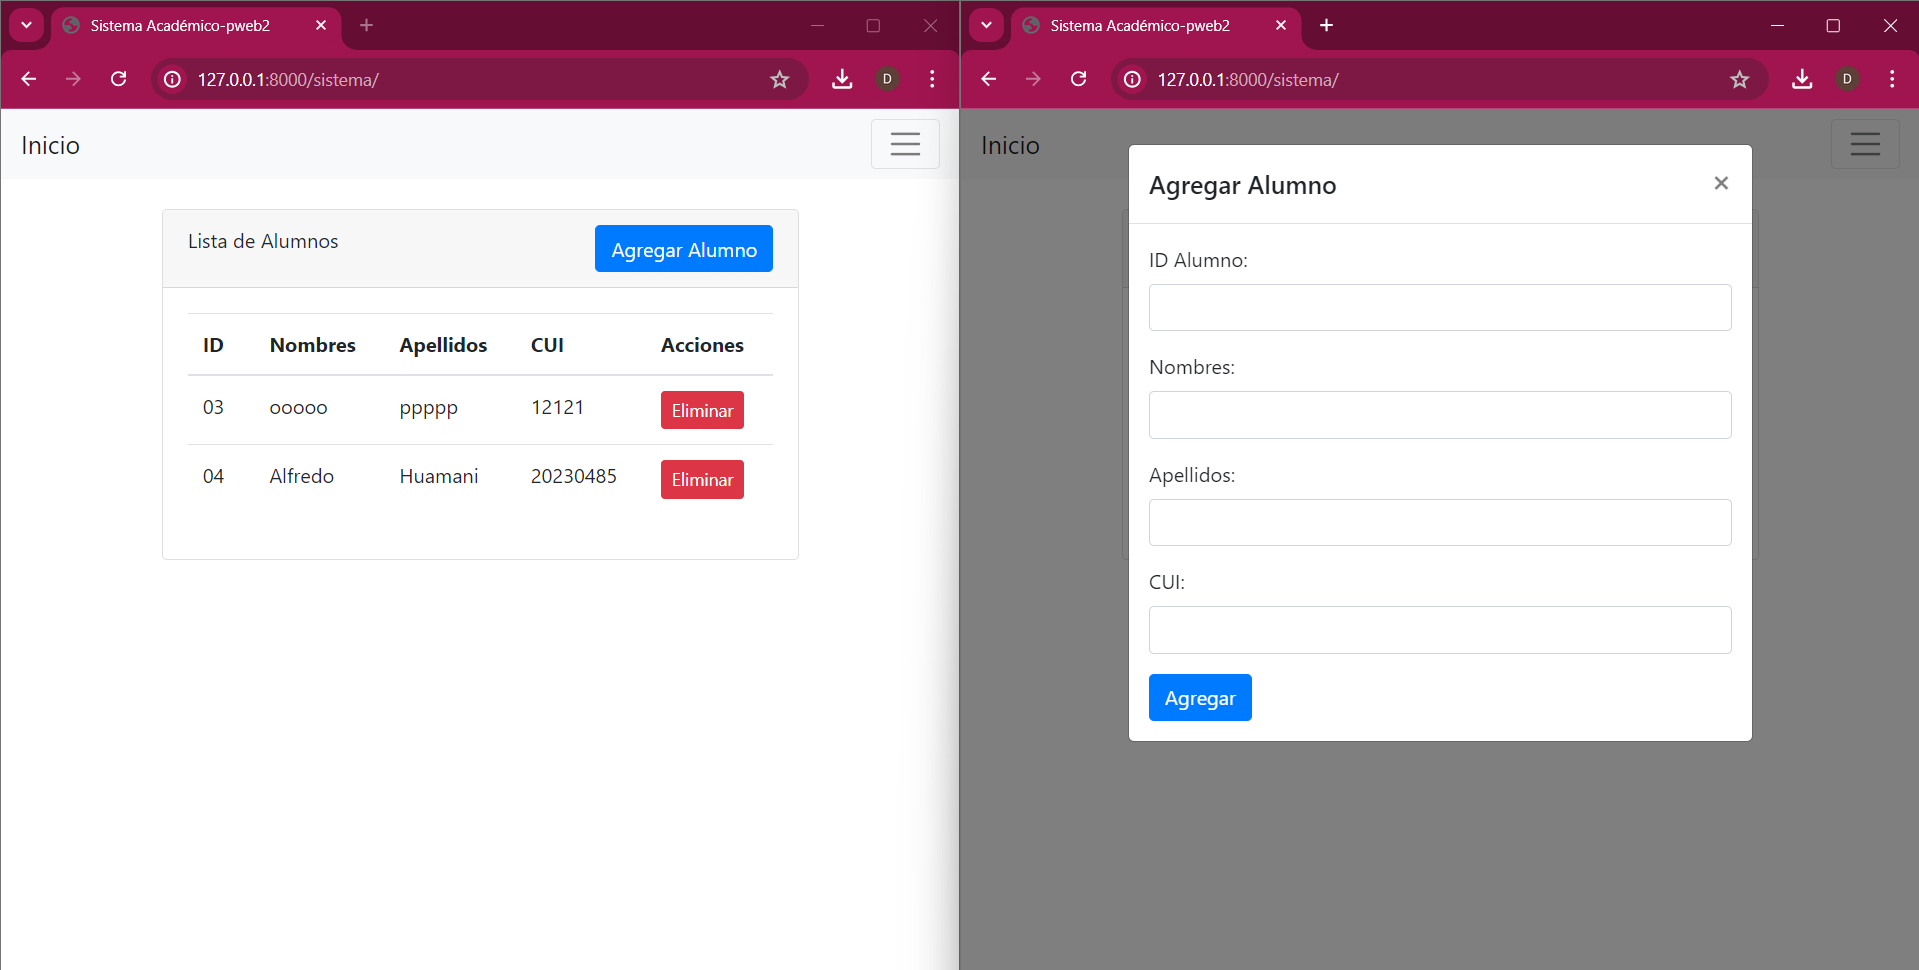
\includegraphics[width=0.9\textwidth]{img/template1.png}
    \caption{Tabla para mostrar alumnos y un boton para añadir y eliminar, el boton de añadir posee campos para llenar para el respectivo modelo alumno}
\end{figure}

\begin{figure}[h!]
    \centering
    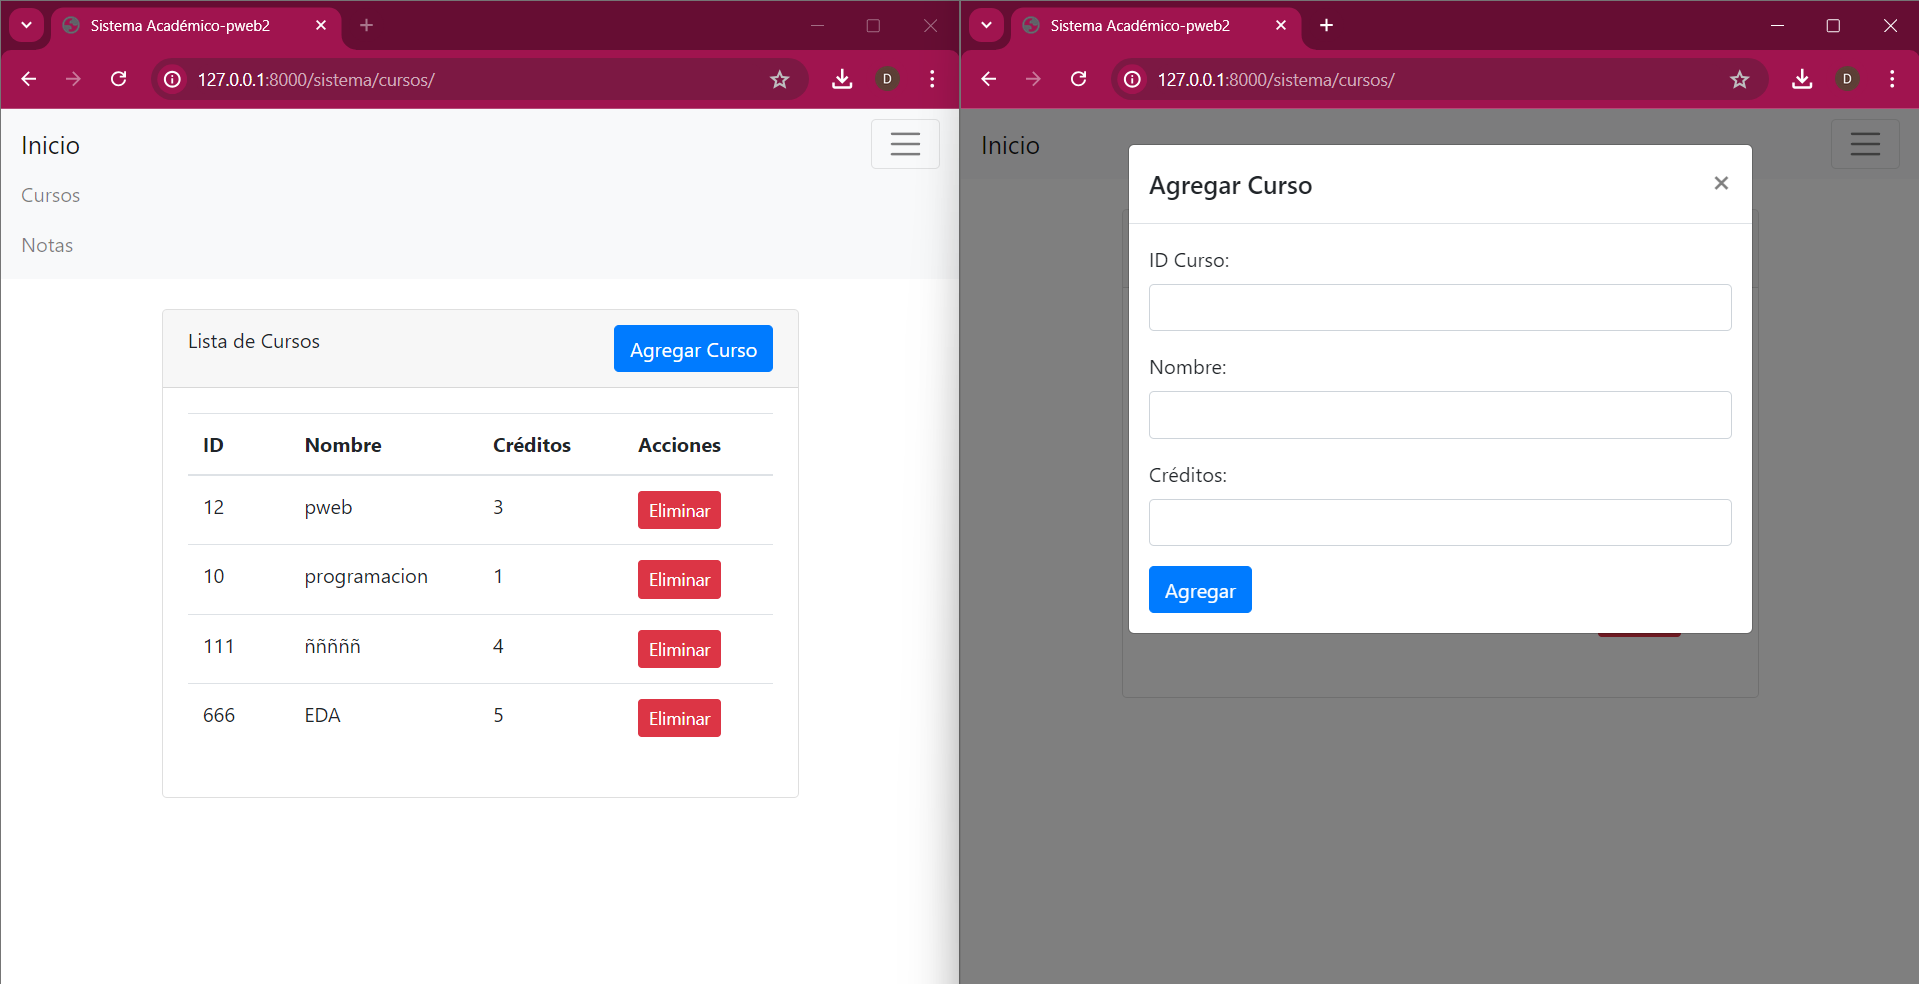
\includegraphics[width=0.9\textwidth]{img/template2.png}
    \caption{Tabla para mostrar cursos y un boton para añadir y eliminar, el boton de añadir posee campos para llenar para el respectivo modelo curso}
\end{figure}

\begin{figure}[h!]
    \centering
    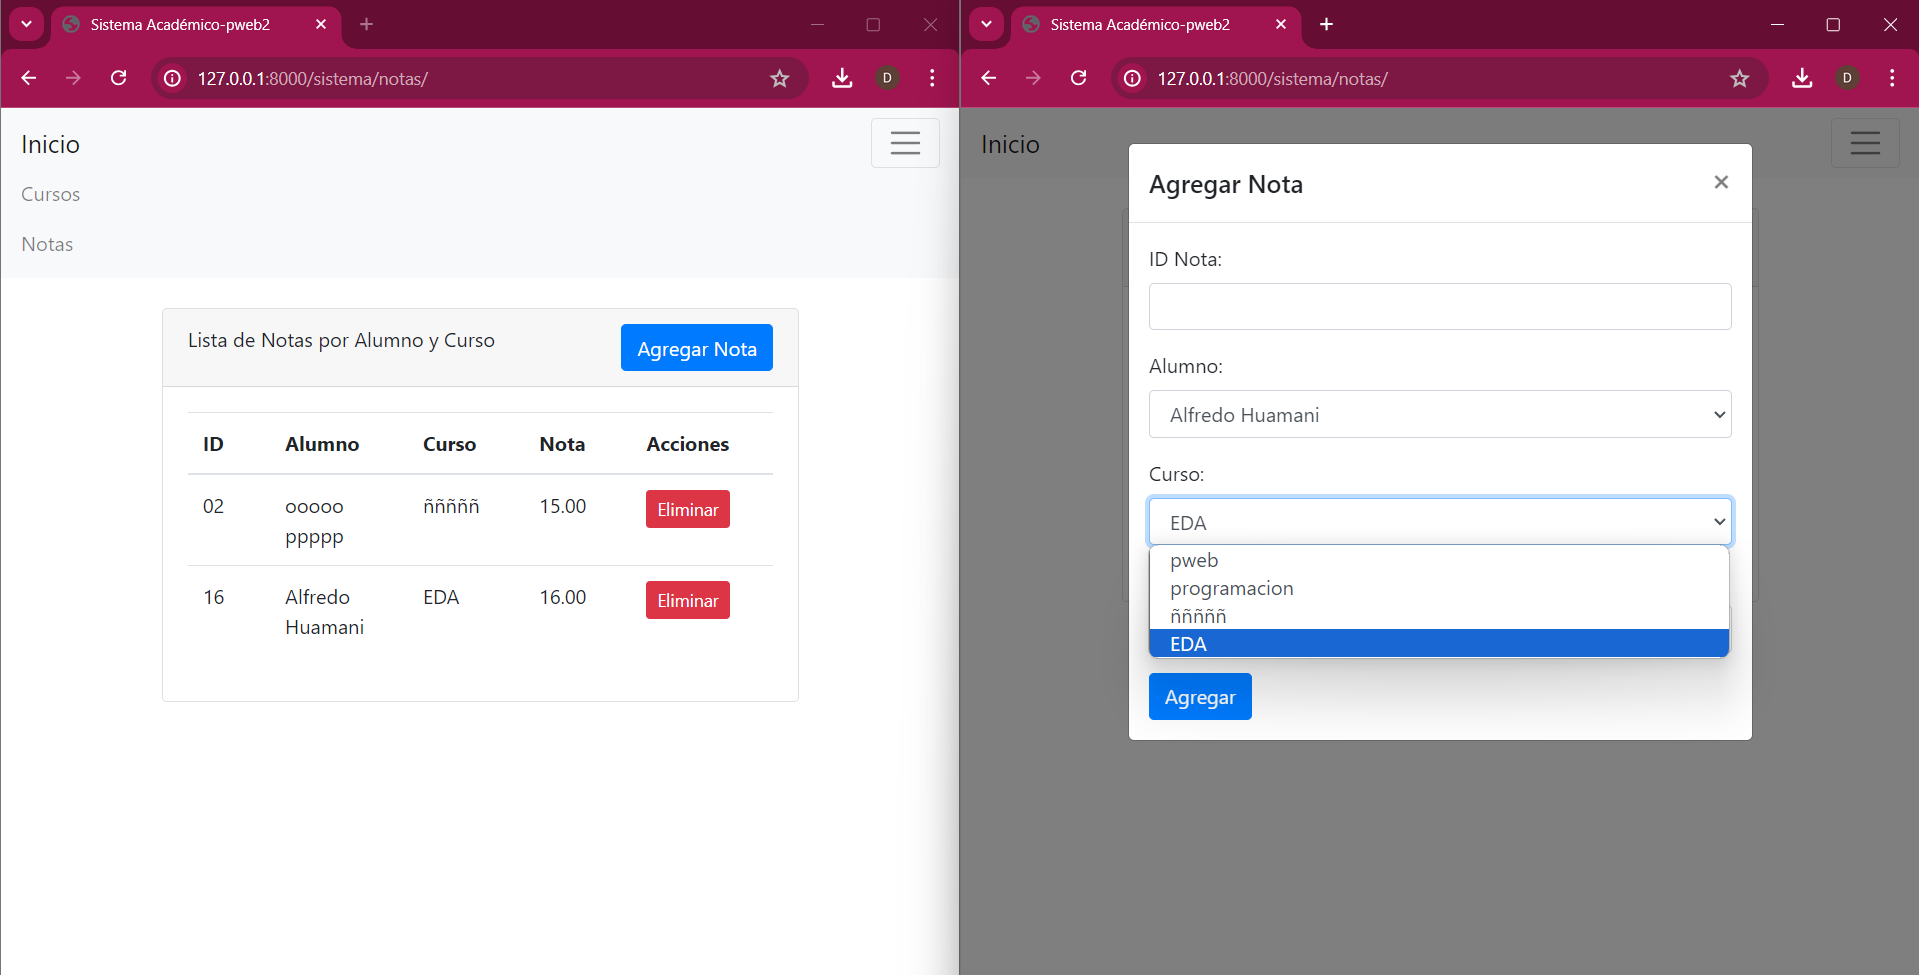
\includegraphics[width=0.9\textwidth]{img/template3.png}
    \caption{Plantilla para relacionar las dos tablas mostradas, cada alumno posee una respectiva nota, al momento de relacionar alumnos con cursos, se muestran los valores de estas tablas}
\end{figure}



	\section{\textcolor{red}{Rúbricas}}
	
	\subsection{\textcolor{red}{Sobre el informe}}
	\begin{table}[H]
		\caption{Tipo de Informe}
		\setlength{\tabcolsep}{0.5em} % for the horizontal padding
		{\renewcommand{\arraystretch}{1.5}% for the vertical padding
		\begin{tabular}{|p{3cm}|p{12cm}|}
			\hline
			\multicolumn{2}{|c|}{\textbf{\textcolor{red}{Informe}}}  \\
			\hline 
			\textbf{\textcolor{red}{Latex}} & \textcolor{blue}{El informe está en formato PDF desde Latex,  con un formato limpio (buena presentación) y facil de leer.}   \\ 
			\hline 
			
			
		\end{tabular}
	}
	\end{table}
	
	\clearpage

	\subsection{\textcolor{red}{Rúbrica para el contenido del Informe y demostración}}
	\begin{itemize}			
		\item El alumno debe marcar o dejar en blanco en celdas de la columna \textbf{Checklist} si cumplio con el ítem correspondiente.
		\item Si un alumno supera la fecha de entrega,  su calificación será sobre la nota mínima aprobada, siempre y cuando cumpla con todos lo items.
		\item El alumno debe autocalificarse en la columna \textbf{Estudiante} de acuerdo a la siguiente tabla:
	
		\begin{table}[ht]
			\caption{Niveles de desempeño}
			\begin{center}
			\begin{tabular}{ccccc}
    			\hline
    			 & \multicolumn{4}{c}{Nivel}\\
    			\cline{1-5}
    			\textbf{Puntos} & Insatisfactorio 25\%& En Proceso 50\% & Satisfactorio 75\% & Sobresaliente 100\%\\
    			\textbf{2.0}&0.5&1.0&1.5&2.0\\
    			\textbf{4.0}&1.0&2.0&3.0&4.0\\
    		\hline
			\end{tabular}
		\end{center}
	\end{table}	
	
	\end{itemize}
	
	\begin{table}[H]
		\caption{Rúbrica para contenido del Informe y demostración}
		\setlength{\tabcolsep}{0.5em} % for the horizontal padding
		{\renewcommand{\arraystretch}{1.5}% for the vertical padding
		%\begin{center}
		\begin{tabular}{|p{2.7cm}|p{7cm}|x{1.3cm}|p{1.2cm}|p{1.5cm}|p{1.1cm}|}
			\hline
    		\multicolumn{2}{|c|}{Contenido y demostración} & Puntos & Checklist & Estudiante & Profesor\\
			\hline
			\textbf{1. GitHub} & Hay enlace URL activo del directorio para el  laboratorio hacia su repositorio GitHub con código fuente terminado y fácil de revisar. &2 &X &2 & \\ 
			\hline
			\textbf{2. Commits} &  Hay capturas de pantalla de los commits más importantes con sus explicaciones detalladas. (El profesor puede preguntar para refrendar calificación). &4 &X &3 & \\ 
			\hline 
			\textbf{3. Código fuente} &  Hay porciones de código fuente importantes con numeración y explicaciones detalladas de sus funciones. &2 &X &2 & \\ 
			\hline 
			\textbf{4. Ejecución} & Se incluyen ejecuciones/pruebas del código fuente  explicadas gradualmente. &2 &X &2 & \\ 
			\hline			
			\textbf{5. Pregunta} & Se responde con completitud a la pregunta formulada en la tarea.  (El profesor puede preguntar para refrendar calificación).  &2 &X &2 & \\ 
			\hline	
			\textbf{6. Fechas} & Las fechas de modificación del código fuente estan dentro de los plazos de fecha de entrega establecidos. &2 &X &2 & \\ 
			\hline 
			\textbf{7. Ortografía} & El documento no muestra errores ortográficos. &2 &X &2 & \\ 
			\hline 
			\textbf{8. Madurez} & El Informe muestra de manera general una evolución de la madurez del código fuente,  explicaciones puntuales pero precisas y un acabado impecable.   (El profesor puede preguntar para refrendar calificación).  &4 &X &3 & \\ 
			\hline
			\multicolumn{2}{|c|}{\textbf{Total}} &20 & &18 & \\ 
			\hline
		\end{tabular}
		%\end{center}
		%\label{tab:multicol}
		}
	\end{table}
	
\clearpage

\section{Referencias}
\begin{itemize}			
	\item \url{https://www.lucidchart.com/pages/es/que-es-un-diagrama-entidad-relacion}
	\item \url{https://docs.djangoproject.com/}
	\item \url{https://www.w3schools.com/python/}
	\item \url{https://www.w3schools.com/django/}

\end{itemize}	
	
%\clearpage
%\bibliographystyle{apalike}
%\bibliographystyle{IEEEtranN}
%\bibliography{bibliography}
			
\end{document}
